%!TEX root=document.tex


\subsection{Pruning-Based Optimizations}
\label{sec:in_memory_execution_engine}
The previous section described techniques to
batch and share computations across queries---however,
if the number of queries is large, this could still 
lead to high execution times, especially
because a lot of resources
are wasted on computing low-utility views. 
In this section, we describe mechanisms to prune away
some aggregate views without complete evaluation. 
Naturally, pruning schemes are {\em approximate},
in that they sometimes incorrectly prune away some
high utility visualizations. 
That said, the visualizations that are displayed
may still be close to high utility 
(which may be good enough for analysts) 
and will certainly be
correct; thus there is still merit to considering approximate schemes.



% The DBMS-backed execution engine from the previous section provides reasonable performance for small datasets.
% However, we find that for medium and large size datasets, the optimized engine take tens to hundreds of produce the top visualizations.
% There are a few reasons for this. (a) Since our engine runs a large number (50-200) queries for each \SeeDB invocation, a large number of scans of the data are performed needlessly; (b) Far too many resources are wasted on low-utility views; and (3) Results of \SeeDB are not available until the entire dataset has been processed.

% To mitigate these drawbacks, we explored a set of pruning strategies to identify and then discard low utility views.
% Pruning low-utility views can allow \SeeDB to reduce the number of queries run on the database, reduce resources spent on eventually-discarded views, and give \SeeDB the ability to return as soon as it has identified the top views.
% In order to evaluate various pruning strategies, we built a simple framework to process records sequentially and perform pruning on the fly.
% We now decribe our test framework and two specific pruning strategies adopted in \SeeDB.

\stitle{Basic Pruning Framework.}
\label{subsec:basic_framework}
We have two kinds of pruning optimizations that we employ.
The first kind is performed {\em online}, i.e., after the
query is provided,
while the second kind is performed {\em offline},
before any queries have been provide.
Our primary focus in this section is the online view pruning;
we will only briefly describe offline view pruning.

Our online view pruning approach involves
multiple {\em phases};
at the end of each phase, we evaluate each aggregate view,
and then decide to prune a number of them, and then keep the rest.
This evaluation and pruning is certainly easy to implement if we were to push these
decisions ``within'' the database layer; however, since
our goal is to operate outside the database without making
any significant changes to the database, we will need some pre-processing
of the underlying tables.
We partition our table horizontally into a number of partitions;
processing each partition corresponds to one of our phases. 
Since we have a collection of these partitions, we can 
choose to operate on them in any random order; if further randomness
is needed, we can preprocess each partition such that the records are internally
in random order.
For each partition in sequence, we update our candidate and target
views for each aggregate view, 
compute the resulting utility, and then 
prune (i.e., discard) or accept (i.e., select to be in those to be displayed) some aggregate views.
When only $k$ aggregate views remain, we can choose to display them
to the analyst (if approximate visualizations are permissible, and latency is paramount),
or we can completely compute the visualizations for those $k$ aggregate views (if not).
We now describe two different schemes used for pruning.
We evaluate both of these schemes in our experiments.

Note that the two pruning schemes described have guarantees
in other settings that do not directly carry over to our setting.
In our evaluation, we show that in spite of this, the pruning schemes
work rather well in practice. 
We can, however, show that as we sample more and more, the estimated utility
$\hat{U}$ can be made to be arbitrarily close to $U$ for all aggregate views.
We show this formally in Section~\ref{sec:discussion}.

\techreport{Algorithm~\ref{algo:custom_exec_engine} shows the outline of our framework.}

\techreport{
\begin{algorithm}[h]
\caption{Pruning Framework}
\label{algo:custom_exec_engine}
\begin{algorithmic}[1]
\State viewsInRunning $\gets$ \{all views\}
\State currPhase $\gets$ 0
\While {currPhase.hasNext()}
\State processNextRecord()
\State updateUtilityEstimates()
\If {currPhase.End()}
\State pruneViews(viewsInRunning)
\State currPhase.Next()
\EndIf
% \If {stoppingCondition.True()}
% \State break
% \EndIf
\EndWhile
\State return viewsInRunning.sort().getTopK()
\end{algorithmic}
\end{algorithm}
}

% Note that we have two alternatives for computing the visualizations for the top-$k$
% views, once $k$ views have been accepted: 
% we can either compute the top-$k$ views to completion (i.e.,
% on the remaining unprocessed records),
% or we can display approximate visualizations for each view, as soon as we ``accept'' them
% as being in the top-$k$. 
% We use the former option as the default, 
% and the latter as an additional optimization that may be employed.
% If at the end of a given phase, \SeeDB\ finds that the views in running satisfy
% the given stopping criteria, e.g., that \SeeDB\ has already identified the
% top-$k$ views, the \SeeDB\ engine can stop processing early.

% \begin{algorithm}
% \caption {ComputeAggregate(Query
% {\it currQuery}, int $d$)}
% %\small 
% \begin{algorithmic}[1] 
% \State int[$d+1$] $currCard$\ \ //All arrays are
% indexed from 1 
% \STATE $currCard[1]$ = ExecuteCellQuery({\it currQuery})  
% \FOR {$i=2$ to $d+1$} 
% \STATE {\it prevQuery} $\leftarrow$ GetPreviousNeighbour($i$-1)\ \ //decrement
% the $(i-1)^{th}$ dimension of {\it currQuery} by stepsize 
% \STATE int[] $prevCard$ = GetAllAggregates({\it prevQuery})
% \STATE $currCard[i]$ = $currCard[i-1]$ + $prevCard[i]$ 
% \ENDFOR 
% \STATE StoreAllAggregates({\it currQuery}, $currCard$) 
% \STATE {\bf return} $currCard[d+1]$
% \end{algorithmic}
% \label{algo:aggregatecomputation}
% % \end {algorithm}
% \mpv{should we remove this?}
% \stitle{Pruning Techniques}: The pruning techniques we discuss next enable \SeeDB\ to discard low-utility views
% early, thus saving computational resources and potentially allowing \SeeDB\ recommend
% views even before all records have been processed.
% To understand the intuition behind the pruning techniques, recall that we define utility of
% view $V_j$ as $ U (V_i) = S ( P[V_i (D_Q)], P[V_i (D)] )$ where $S$ is a distance function measuring
% the distance between the target and comparison distributions, $P[V_i (D_Q)]$ and $P[V_i (D)]$.
% Let the total number of records in the input be denoted by $R$ and the total records
% read by phase $j$ as $R_j$. 
% Once $R_j$ records have been read in, we can estimate target and comparison 
% distributions, $\widetilde{P}^j[V_i (D_Q)]$ and $\widetilde{P}^j[V_i (D)]$.
% As \SeeDB\ processes larger portions of the file, these estimates become more accurate. 
% As one might expect:

% $$\lim_{R_j \rightarrow R}\widetilde{P}^j[V_i (D_Q)] \rightarrow P[V_i (D_Q)] \cap 
% \widetilde{P}^j[V_i (D)] \rightarrow P[V_i (D)] $$

% metric discussed in Section \ref{} are of the form $\mathcal{F}:
% (\mathcal{R}^p, \mathcal{R}^p) \rightarrow \mathcal{R}$, i.e. they are functions
% measuring the distance between the target and comparison distributions of a view.
% For view $V_j$ let $\mathcal{P}^j_T$ and $\mathcal{P}^j_C$ respectively denote the 
% target and comparison view of $V_j$.

% Therefore, as we process records in every phase $j$, we can keep running estimates of the
% view distributions as well as view utilities, $\widetilde{U}^j(V_i)$.
% Moreover, {\it we can use these estimates to perform the pruning of low utility views}.
% In this paper, we propose and evaluate two different strategies
% to perform the pruning of views based on utility estimates. 
% The first strategy is based on top-$k$ algorithms that use confidence intervals 
% and the second is based on an adaptation of the Multi-Armed Bandit problem.

% of the view distributions $\widetilde{\mathcal{P}}^{i,j}_T$ and $\widetilde{\mathcal{P}}^{i,j}_C$
% and estimates of the utility $\mathcal{F}(\widetilde{\mathcal{P}}^{i,j}_T, 
% \widetilde{\mathcal{P}}^{i,j}_C)$.

% The general idea is to keep running estimates of utility for each view, and
% perform pruning of low utility views based on these estimates.
% To implement a pruning strategy, we merely specify two things: (1)
% statistics to track for each view, and 
% (2) the rule used to prune views at the end of a phase.
% An important side effect of our implementation is that
% as we scan more data from the file, our estimates of utilities become more
% accurate.

% 
% \begin{itemize}
% \item The first two strategies are based on confidence interval-based top-$k$ algorithms.
% That is, at the end of each phase, confidence intervals are updated for all
% the views still in the running and we prune views based on overlap
% with the top-$k$ confidence intervals.
% % and if the upper-bound for any of them
% % is lower than the lower-bound for confidence intervals of $k$ or more other views,
% % then those views are discarded.
% \begin{denselist}
% \item The first uses worst-case confidence intervals based on the
% Hoeff\-ding-Serfling inequality~\cite{serfling1974probability}, 
% which is a generalization of Hoeffding's inequality~\cite{hoeffding1963probability}
% when a number of samples are randomly chosen without replacement
% from the same set.
% These confidence intervals are necessarily more conservative.
% \item The second assumes that the underlying probability distribution is
% Gaussian and uses 95\% confidence intervals~\cite{all-of-statistics}.
% These confidence intervals are more ``aggressive'' compared to those derived
% from the Hoeffding inequality.
% (For experiments evaluating this assumption, see Section~\ref{sec:evaluating_normal}.) 
% \end{denselist}
% \item The last strategy is based on an adaptation of Multi-Armed Bandit (MAB)
% algorithms for top-$k$ arm identification~\cite{}. 
% Multi-Armed Bandit algorithms are well-studied in the field of stochastic
% control; in our scenario, the arms are the views, and pulling an arm corresponds
% to updating a view's utility.
% \end{itemize}


\stitle{Confidence Interval-Based Online Pruning.}
\label{sec:confidence_interval}
Our first pruning scheme uses worst-case statistical confidence intervals.
Our scheme is as follows: during execution,
we keep an estimate of the mean utility for every aggregate view $V_i$ and a
confidence interval around that mean.
That is, for every view $V_i$ we track its mean utility $u_i$, and a
confidence interval around the mean, $u_i \pm c_i$. 
At the end of a phase, we use the following rule to prune low-utility
views:
{\em If the upper bound of the utility of view $V_i$ is lesser
than the lower bound of the utility of $k$ or more views, then $V_i$ is discarded.}

\begin{figure}[h]
\vspace{-10pt}
\centerline{
\hbox{\resizebox{8cm}{!}{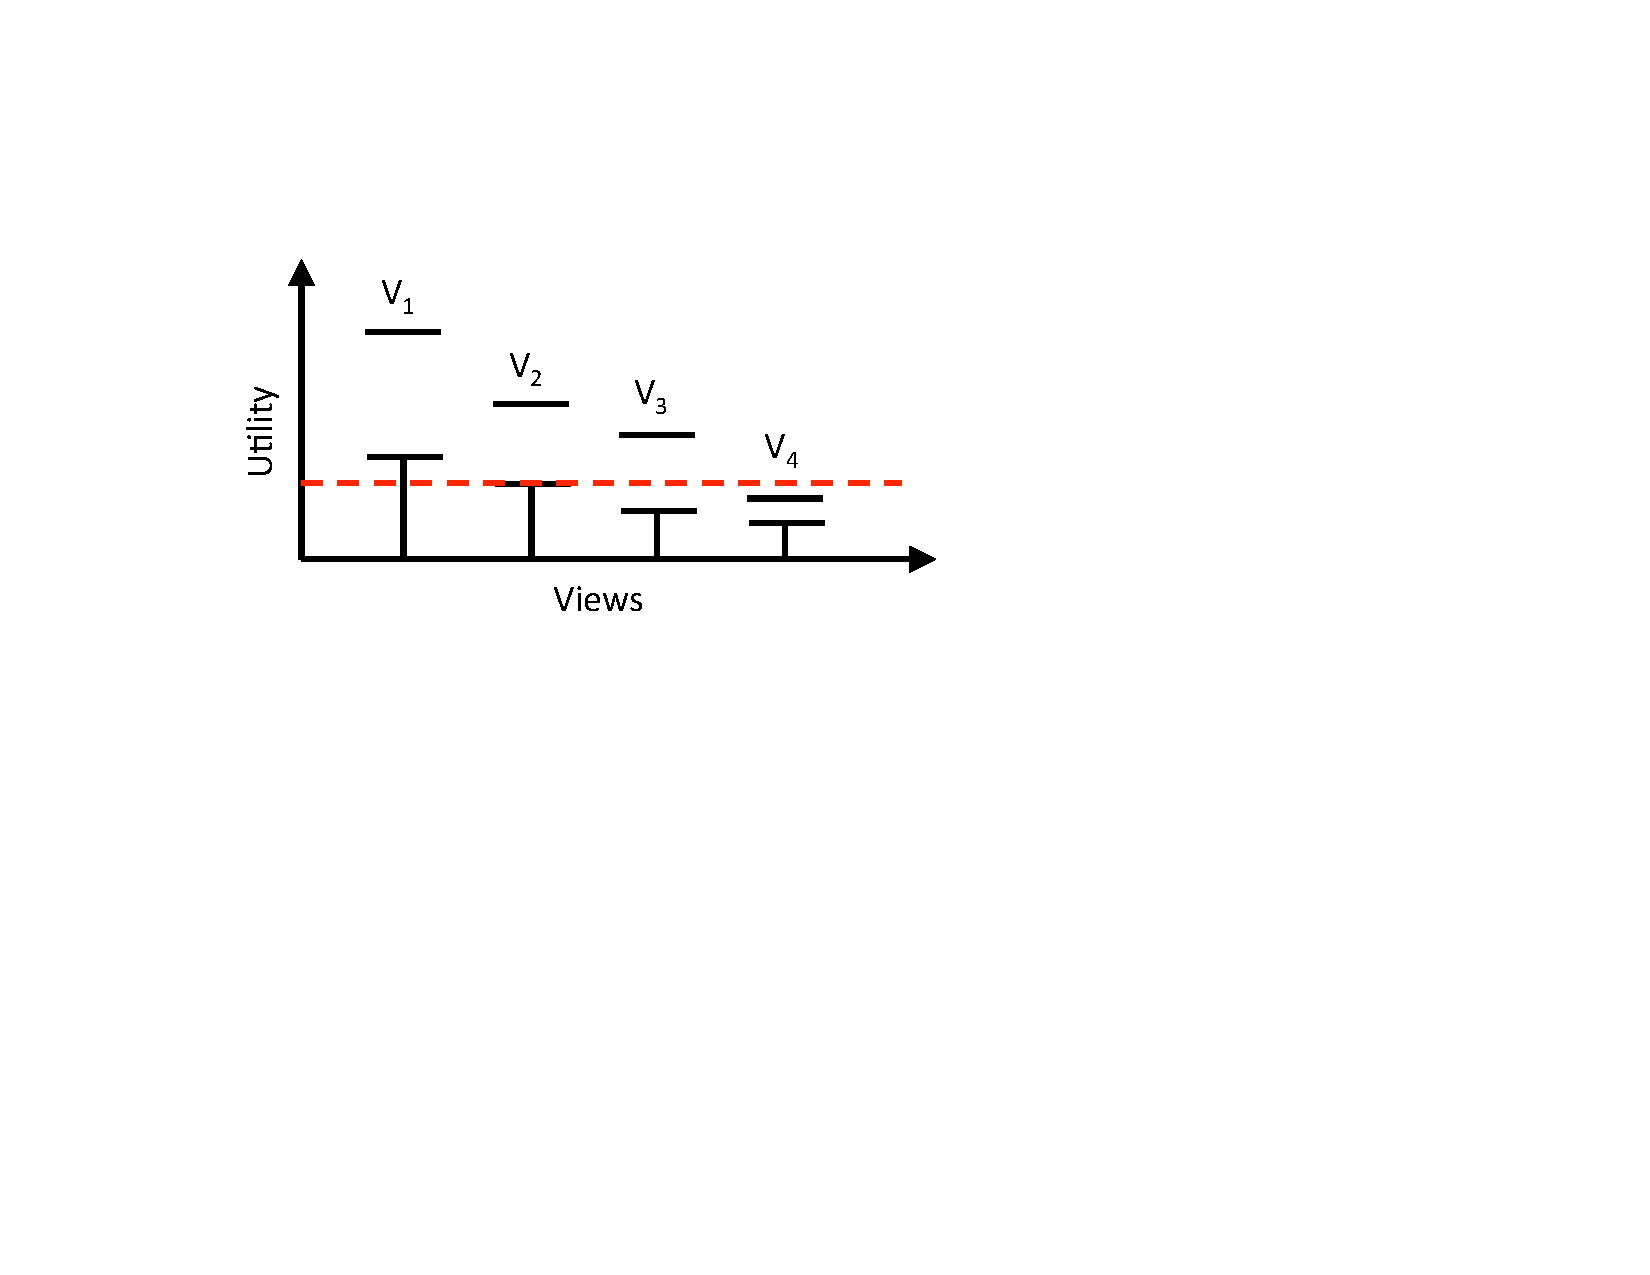
\includegraphics[trim=10mm 100mm 55mm 35mm, 
clip=true]{Images/confidence_pruning.pdf}}}}
\vspace{-20pt}
\caption{Confidence Interval based Pruning}
\label{fig:conf_interval}
\vspace{-15pt}
\end{figure}

To illustrate, suppose a dataset has 4 views $V_1$ to $V_4$ and we want to find the top-$2$ views.
Further suppose that at the end of phase $p$,
$V_1$-$V_4$ have confidence intervals as shown in Figure \ref{fig:conf_interval}.
Views $V_1$ and $V_2$ have the highest estimates for utility so far.
Consider view $V_3$; we see that its confidence interval overlaps with the
confidence intervals of the current top views, making it possible
that $V_3$ will be in the final top views. On the other hand, the confidence
interval for $V_4$ lies entirely below the lowerbounds of $V_1$ and $V_2$.
Since we can claim with high probability
that the utility of $V_4$ lies within its confidence interval, it follows that
with high probability, $V_4$'s utility will be lower than that of both $V_1$ and
$V_2$, and it will not appear in the top-$2$ views.
\papertext{Pseudocode for our pruning scheme can be found in our technical report~\cite{seedb-tr}.}
\techreport{We state the algorithm formally in
Algorithm~\ref{algo:ci_based_pruning}.}

\techreport{
\begin{algorithm}
\caption{Confidence Interval Based Pruning}
\label{algo:ci_based_pruning}
\begin{algorithmic}[1]
\State viewsInRunning.sortByUpperbound()
\State topViews $\gets$ viewsInRunning.getTopK()
\State lowestLowerbound $\gets$ min(lowerbound(topViews))
\For {view $\not \in$ topViews}
\If {view.upperbound < lowestLowerbound}
\State viewsInRunning.remove(view)
\EndIf
\EndFor
\end{algorithmic}
\end{algorithm}
}

We use {\it worst case} confidence intervals as derived from
the Hoeffding-Serfling inequality~\cite{serfling1974probability}.
The inequality states that if we are given $N$ values $y_1, \ldots, y_N$ in 
$[0, 1]$ with average $\mu$, and we have have drawn $m$ values without replacement, $Y_1, \ldots, Y_m$, 
then we can calculate a running confidence interval around the current mean 
of the $m$ values such that the actual mean of the $N$
is always within this confidence interval with a probability of $1 - \delta$:
\begin{theorem}
\label{thm:hs}
% Let $\calY = y_1,$ $\ldots,$ $y_N$ be a set of $N$ 
% values in $[0,1]$ with average value
% $\frac1N \sum_{i=1}^N y_i = \mu$.
% Let $Y_1,\ldots,Y_N$ be a 
% sequence of random variables drawn from $\calY$ without
% replacement.
Fix any $\delta > 0$. For $1 \le m \le N-1$, define
{\small $$
\varepsilon_m = \sqrt{\frac{(1-\frac{m-1}N)(2\log \log (m) + \log(\pi^2/3\delta))}{2m}}.
$$
$$
\textrm{Then:} \ \   \Pr\left[ \exists m, 1 \le m \le N : 
  \left|\frac{\sum_{i=1}^m Y_i}{m} - \mu\right| > \varepsilon_m \right] 
\le \delta.
$$
}

\end{theorem}
In our setting, each $Y_i$ corresponds to the an estimate of utility computed based on the
records seen so far. 
% estimates of utility that we 
% have obtained based on the set of records seen thus far. 
% Therefore, to apply this pruning strategy, we track the current estimates of
% view utilities at each step and use the above confidence interval calculation
% to perform pruning at the end of every phase.

% Note that in this setting, we are assuming that since the
% utility estimate at any stage of processing is in $[0, 1]$, 
% the $Y_i$ values, i.e., the incremental contributions to the utility
% that come from reading each record, are also between $[0, 1]$,
% and are independent of the current value of the utility. 
% This is is not true in our setting, 
% because the utility function could be arbitrary.
% Thus, the theoretical guarantees do not directly apply to our setting. 

% \stitle{Normal Confidence Intervals.} In this scheme, we assume that the utility
% distributions for each view are Gaussian and apply the standard confidence
% intervals to our utility measurements.
% % We describe the equations first assuming that
% % when every time a record is read, for every view,
% % a utility value is ``sampled''
% % from a normal distribution. (This assumption is not
% % quite correct; we will discuss this  below.)

% Consider a specific view $V_i$. 
% If the mean utility across the sampled records 
% (i.e., the records read thus far) is $\mu$,
% and the variance in the utility of the sampled records
% is $\sigma$, then, we have:
% \begin{align}
% CI & = \mu \pm z \times \frac{\sigma}{\sqrt{m}}
% \end{align}
% Thus, the CI (or confidence interval) is 
% a confidence interval centered around $\mu$, 
% and depends on $\sigma$. 
% It additionally depends on the number of records
% read thus far, $m$,
% and $z$, the factor that depends on our confidence interval threshold.
% For instance, for a 95\% confidence interval, $z = 1.96$.

% We note that the assumption that we are drawing from a normal distribution is
% not quite accurate since our samples vary in size and are not independent.
% As a result, we make two simple adjustments to the confidence interval
% calculations that are described in Appendix~\ref{sec:ci_pruning}.
% In Section \ref{sec:experiments}, we show experimentally on multiple datasets
% that our confidence interval calculations accurately capture utility and can be used to
% perform pruning with high confidence.






% \stitle{Normal Confidence Intervals.}
% As described above, we must specify
% a set of statistics to track for each view and a rule that is used to
% prune views based on the statistic.
% For confidence interval based pruning, the statistics we track are the mean, 
% variance, and confidence intervals of the view utility.
% As \SeeDB\ reads each record, it updates the data
% distributions for all views and calculates the current utility of each view. 
% Using past measures of utility, \SeeDB\ also tracks the mean,
% variance and confidence intervals for the utility of each view.
% % At the end of a phase, \SeeDB\ uses the following rule for pruning low-utility
% % views (stated more formally below): {\it if the upperbound on the utility
% % of view $v_i$ is lesser than the least lowerbound on the utility of the
% % top-$k$ views, view $v_i$ is discarded.}

% % Let us dive deeper into this pruning rule.
% Note that as we sequentially read records from a file, we are
% approximating a sampling process (remember that the records are in random order).
% For instance, suppose that we have read 10K records from a 1M record file.
% In this case, the records 1 -- 10K constitute a 1\% sample of the entire file.
% When we read the next say 10 records, the records 1 -- 10,010 constitute an
% incrementally larger sample of the underlying file.
% Thus, as we read more data from the file, we obtaining a large
% number of samples from the underlying data (notice however, that these samples
% are not independent).

% Since we are generating a large number of samples from a population, we can
% invoke a well-studied concept in statistics called the ``sampling distribution.'' 
% A sampling distribution for a statistic $S$ is the distribution of
% $S$ generated by taking a large number of samples of a fixed size and computing
% the statistic $S$ on each sample.
% In our case, the population we draw from is the set of all records in the file
% and our samples are the increasingly larger sets of records that we are reading in.
% The statistic $S$ that we are computing is the view utility (we
% compute a utility value for each view).
% Now, the sampling distribution of the {\it mean} has been well studied and it
% has been proven that the mean of the sampling distribution is equal to the mean of the
% population and the standard error of the sampling distribution is equal to the
% standard error of the population divided by the square root of the sample size. 
% These two formulas are shown in Equations \ref{eq:mean} and \ref{eq:variance}.
% Similarly, if we know the mean and standard error of the sampling distribution,
% we can compute a confidence interval around the population mean. This is shown
% in Equation \ref{eq:confidence_interval} where $z$ is the factor that depends on the
% confidence threshold we are aiming for and $N$ is the number of items
% in each sample.

% \begin{eqnarray}
% \label{eqnarray:mean_and_variance}
% \mu_M = \mu \label{eq:mean}\\
% \sigma_{M} = \frac{\sigma}{\sqrt{N}} \label{eq:variance}\\
% CI = \mu_M \pm z \ast \frac{\sigma_M}{\sqrt{N}}\label{eq:confidence_interval}
% \end{eqnarray}

% If we were modeling the mean of our samples instead of the utility, we could use
% the above result directly.
% However, we find that with a few minor modifications, we can use the confidence
% interval bounds shown above.
% The first modification we make has to do with how we define utility.
% Remember from Section \ref{sec:problem_definition} that the utility of a view is
% defined as the distance between two distributions: the distribution of aggregate values for the
% target view and the distribution of aggregate values for the comparison view.
% These distributions are in turn tied to the number of distinct groups present in
% each dimension attribute.
% For our purposes, it means that if a dimension attribute has $n$ distinct
% groups, then a sample with $x$ rows gives us approximately $\frac{x}{n}$ values
% for each group (assuming uniform distribution).
% Said another way, a sample with $x$ rows for the purpose of computing utility is
% really only a sample of $\frac{x}{n}$ rows.
% So the first modification we make to Equation \ref{eq:confidence_interval} is to
% replace $N$ by $\frac{N}{G_{max}}$ where $G_{max}$ is the maximum number of
% distinct groups present in any dimension attribute.
% Second, we observe that the sampling distribution applies to the case where
% samples are of the same size and are independently generated.
% This is not true in our algorithm; therefore, to compensate, make two
% conservative modifications: we set $N$ to the number of rows that
% have been read in the previous phase (remember that pruning happens at the end
% of every phase) and we set the $z$ parameter to a value $\geq$ 1.96 (the normal
% 95\% confidence interval value). These modifications ensure (as we will show
% empirically in Section \ref{sec:experiments}) that the confidence intervals
% always contain the mean and continually shrink as we read in more data.

% As shown in Line 12 of Algorithm \ref{algo:custom_exec_engine},
% when a phase ends, we clear all statistics collected in that phase; we do not
% want less accurate estimates from previous phases to contaminate the more
% accurate estimates from subsequent phases. \agp{deal with this.}






% Now that we have a way of finding confidence intervals, we elaborate on how we
% use them to perfom pruning.
% Suppose at the end of phase $p$ the confidence intervals for the views in
% running have values shown in Figure \ref{fig:conf_interval} and we want to
% identify the two views with the highest utility.
% Consider view $V_3$, we see that its confidence interval overlaps with the
% confidence intervals of the current top views $V_1$ and $V_2$, making it likely
% that $V_3$ will be in the final top views. On the other hand, the confidence
% interval for $V_4$ lies entirely below the lowest bound of the top two
% intervals.
% Since we can claim with high probability (depending on the confidence threshold)
% that the utility of $V_4$ lies within its confidence interval, it follows that
% with high probability, $V_4$ will not appear in the top-$2$ views.
% This is essentially our pruning rule. 
% 



\stitle{Multi-Armed Bandit Online Pruning.}
\label{sec:multi_armed_bandit}
Our second pruning scheme uses Multi-Armed Bandit (MAB)~\cite{bandits} policies.\techreport{The setting of MAB is as follows: a gambler is faced with several slot
machines (``one-armed bandit''s), each of which has an underlying 
(unknown) reward distribution. 
Every play results in a reward from the corresponding machine's
reward distribution.
The goal is to devise a {\it strategy} of which machine to play
at each turn in order to maximize the reward~\cite{bandits}.}
A recently-studied variation of MAB focuses on finding the arms with the highest
mean rewards~\cite{BubeckWV13}.
This variation is similar to the problem addressed by \SeeDB: each possible view 
can be thought of as a one-armed bandit and our goal is find the views with the 
highest reward (i.e. utility).
We therefore adapt the Successive Accepts and Rejects algorithm from \cite{BubeckWV13} 
to find arms with the highest mean reward. 
\techreport{Algorithm~\ref{algo:mab_based_pruning} shows the pseudocode for our pruning technique.}
% As before, the processing of the input table is divided into phases.
% In every phase, \SeeDB\ reads in new records and updates the distributions and utilities
% for every view in the running.
At the end of every phase, all active views are ranked in order of their utility means. 
We then compute two special differences between the utility means: $\Delta_1$
is the difference between the highest mean and the $k+1$st highest mean, and
$\Delta_n$ is the difference between the lowest mean and the $k$th highest mean.
If $\Delta_1$ is greater than $\Delta_n$, the view with the highest mean is
``accepted'' as being part of the the top-$k$ (and it no longer participates
in pruning computations).
On the other hand, if $\Delta_n$ is higher, the view with the lowest mean is discarded
from the set of views in the running.
\cite{BubeckWV13} proves that under certain assumptions about reward distributions,
the above technique identifies the top-$k$ arms with high probability.


% In MAB, each pull of an arm corresponds to a drawing from a sample
% the underlying probability distribution of that arm.
% In our case, each new record updates the utilities for all views and
% each resulting updated utility can be thought of as a sample from the
% utility distribution of that view.

% In applying MAB techniques to our problem setup, we make two assumptions:
% (1) although the utility of a
% view is ultimately a single value, we can approximate it as a probability
% distribution that is normally distributed around the true utility, and 
% (2) our running estimate of utility after reading $i$
% records is a sample derived from the above utility distribution.

\techreport{
\begin{algorithm}
\caption{MAB Based Pruning}
\label{algo:mab_based_pruning}
\begin{algorithmic}[1]
\State viewsInRunning.sortByUtilityMean()
\State \{$\bar{u}_{i}$\} $\gets$ sorted utility means
\State $\Delta_1$ $\gets$ $\bar{u}_{1}$ - $\bar{u}_{k+1}$
\State $\Delta_n$ $\gets$ $\bar{u}_{k}$ - $\bar{u}_{n}$
\If {$\Delta_1$ < $\Delta_n$}
\State viewsInRunning.acceptTop()
\Else
\State viewsInRunning.discardBottom()
\EndIf
\end{algorithmic}
\end{algorithm}
}





% \techreport{\cite{BubeckWV13} provides bounds on the optimality of this heuristic for the
% MAB setting.
% Since our problem setup isn't exactly the same, the optimality bounds don't
% transfer directly.
% However, as we show in the experimental section, the MAB heuristic performs well
% on real datasets.}